% Options for packages loaded elsewhere
\PassOptionsToPackage{unicode}{hyperref}
\PassOptionsToPackage{hyphens}{url}
%
\documentclass[
  english,
  man,floatsintext]{apa6}
\usepackage{lmodern}
\usepackage{amssymb,amsmath}
\usepackage{ifxetex,ifluatex}
\ifnum 0\ifxetex 1\fi\ifluatex 1\fi=0 % if pdftex
  \usepackage[T1]{fontenc}
  \usepackage[utf8]{inputenc}
  \usepackage{textcomp} % provide euro and other symbols
\else % if luatex or xetex
  \usepackage{unicode-math}
  \defaultfontfeatures{Scale=MatchLowercase}
  \defaultfontfeatures[\rmfamily]{Ligatures=TeX,Scale=1}
\fi
% Use upquote if available, for straight quotes in verbatim environments
\IfFileExists{upquote.sty}{\usepackage{upquote}}{}
\IfFileExists{microtype.sty}{% use microtype if available
  \usepackage[]{microtype}
  \UseMicrotypeSet[protrusion]{basicmath} % disable protrusion for tt fonts
}{}
\makeatletter
\@ifundefined{KOMAClassName}{% if non-KOMA class
  \IfFileExists{parskip.sty}{%
    \usepackage{parskip}
  }{% else
    \setlength{\parindent}{0pt}
    \setlength{\parskip}{6pt plus 2pt minus 1pt}}
}{% if KOMA class
  \KOMAoptions{parskip=half}}
\makeatother
\usepackage{xcolor}
\IfFileExists{xurl.sty}{\usepackage{xurl}}{} % add URL line breaks if available
\IfFileExists{bookmark.sty}{\usepackage{bookmark}}{\usepackage{hyperref}}
\hypersetup{
  pdftitle={Dwell times disambiguate preschoolers' attention to motion versus goal structure as dynamic action unfolds},
  pdflang={en-EN},
  pdfkeywords={event segmentation, event processing, goal structure, dwell-time paradigm, dynamic action},
  hidelinks,
  pdfcreator={LaTeX via pandoc}}
\urlstyle{same} % disable monospaced font for URLs
\usepackage{graphicx}
\makeatletter
\def\maxwidth{\ifdim\Gin@nat@width>\linewidth\linewidth\else\Gin@nat@width\fi}
\def\maxheight{\ifdim\Gin@nat@height>\textheight\textheight\else\Gin@nat@height\fi}
\makeatother
% Scale images if necessary, so that they will not overflow the page
% margins by default, and it is still possible to overwrite the defaults
% using explicit options in \includegraphics[width, height, ...]{}
\setkeys{Gin}{width=\maxwidth,height=\maxheight,keepaspectratio}
% Set default figure placement to htbp
\makeatletter
\def\fps@figure{htbp}
\makeatother
\setlength{\emergencystretch}{3em} % prevent overfull lines
\providecommand{\tightlist}{%
  \setlength{\itemsep}{0pt}\setlength{\parskip}{0pt}}
\setcounter{secnumdepth}{-\maxdimen} % remove section numbering
% Make \paragraph and \subparagraph free-standing
\ifx\paragraph\undefined\else
  \let\oldparagraph\paragraph
  \renewcommand{\paragraph}[1]{\oldparagraph{#1}\mbox{}}
\fi
\ifx\subparagraph\undefined\else
  \let\oldsubparagraph\subparagraph
  \renewcommand{\subparagraph}[1]{\oldsubparagraph{#1}\mbox{}}
\fi
% Manuscript styling
\usepackage{upgreek}
\captionsetup{font=singlespacing,justification=justified}

% Table formatting
\usepackage{longtable}
\usepackage{lscape}
% \usepackage[counterclockwise]{rotating}   % Landscape page setup for large tables
\usepackage{multirow}		% Table styling
\usepackage{tabularx}		% Control Column width
\usepackage[flushleft]{threeparttable}	% Allows for three part tables with a specified notes section
\usepackage{threeparttablex}            % Lets threeparttable work with longtable

% Create new environments so endfloat can handle them
% \newenvironment{ltable}
%   {\begin{landscape}\begin{center}\begin{threeparttable}}
%   {\end{threeparttable}\end{center}\end{landscape}}
\newenvironment{lltable}{\begin{landscape}\begin{center}\begin{ThreePartTable}}{\end{ThreePartTable}\end{center}\end{landscape}}

% Enables adjusting longtable caption width to table width
% Solution found at http://golatex.de/longtable-mit-caption-so-breit-wie-die-tabelle-t15767.html
\makeatletter
\newcommand\LastLTentrywidth{1em}
\newlength\longtablewidth
\setlength{\longtablewidth}{1in}
\newcommand{\getlongtablewidth}{\begingroup \ifcsname LT@\roman{LT@tables}\endcsname \global\longtablewidth=0pt \renewcommand{\LT@entry}[2]{\global\advance\longtablewidth by ##2\relax\gdef\LastLTentrywidth{##2}}\@nameuse{LT@\roman{LT@tables}} \fi \endgroup}

% \setlength{\parindent}{0.5in}
% \setlength{\parskip}{0pt plus 0pt minus 0pt}

% \usepackage{etoolbox}
\makeatletter
\patchcmd{\HyOrg@maketitle}
  {\section{\normalfont\normalsize\abstractname}}
  {\section*{\normalfont\normalsize\abstractname}}
  {}{\typeout{Failed to patch abstract.}}
\makeatother
\shorttitle{Preschoolers' attention to motion versus goal structure}
\author{Jessica E. Kosie\textsuperscript{1,2}\ \& Dare Baldwin\textsuperscript{2}}
\affiliation{
\vspace{0.5cm}
\textsuperscript{1} Department of Psychology, Princeton University\\\textsuperscript{2} Department of Psychology, University of Oregon}
\authornote{

Correspondence concerning this article should be addressed to Jessica E. Kosie, Department of Psychology, Princeton University, Princeton, NJ 08540 USA. E-mail: jkosie@princeton.edu}
\keywords{event segmentation, event processing, goal structure, dwell-time paradigm, dynamic action\newline\indent Word count: X}
\usepackage{lineno}

\linenumbers
\usepackage{csquotes}
\ifxetex
  % Load polyglossia as late as possible: uses bidi with RTL langages (e.g. Hebrew, Arabic)
  \usepackage{polyglossia}
  \setmainlanguage[]{english}
\else
  \usepackage[shorthands=off,main=english]{babel}
\fi
\newlength{\cslhangindent}
\setlength{\cslhangindent}{1.5em}
\newenvironment{cslreferences}%
  {\setlength{\parindent}{0pt}%
  \everypar{\setlength{\hangindent}{\cslhangindent}}\ignorespaces}%
  {\par}

\title{Dwell times disambiguate preschoolers' attention to motion versus goal structure as dynamic action unfolds}

\date{}

\abstract{
We harnessed Hard, Recchia, \& Tversky's (2011) dwell-time paradigm to tease apart the influence of motion patterns and goal structure on children's analysis of events as dynamic action unfolds. Ninety-two preschoolers (aged 2.5-4.5 years) advanced at their own pace through one of three slideshows, all depicting an actor reaching toward and retrieving a ball. However, motion patterns differed for one slideshow (straight reach) relative to the other two (arcing reach), and one of the arcing reach slideshows depicted a violation of canonical goal-related motion (arcing reach in the absence of any barrier). Dwell-time patterns revealed comparable segmental analyses across all three slideshows, confirming children's tendency to privilege goal structure over motion characteristics in their moment-to-moment analysis of continuously unfolding activity sequences.
}

\begin{document}
\maketitle

\hypertarget{introduction}{%
\section{Introduction}\label{introduction}}

Our everyday experience of the world centers on a sense of discrete events that occur across time. For example, we might experience a simple trip to the grocery store as a series of events that include parking the car, entering the store,being bumped into by a distracted shpper, putting groceries into a cart, paying the cashier, navigating a crowded parking lot, and loading up the trunk. Interestingly, the activity actually underlying this experience of events tends to be complex, dynamic, and evanescent. How do we transform the continuous, multi-modal stream that actually occurs into the experience of an event sequence? Answering this question has proven to be surprisingly challenging (Baldwin \& Baird, 1999, 2001; Kurby \& Zacks, 2008; Newtson, Engquist, \& Bois, 1977; Zacks, Speer, Swallow, Braver, \& Reynolds, 2007; Zacks \& Tversky, 2001). Even more challenging is to answer how infants and young children come to acquire adult-like skill at rendering continuously flowing experience in terms of event sequences. One challenge that has slowed progress on these issues is methodological: a dearth of available techniques for examining children's processing as information unfolds across time. In this paper, we showcare a valuable new method for this purpose, and report novel information about the nature of event-processing skill in preschool-aged children.

A recent surge of research on adults' event processing offers starting information about the perceptual and cognitive skills at play in this mental rendering process. For one, adult observers display high levels of agreement when asked to consciously report on the location of event boundaries in continuously streaming activity sequences (Newtson, 1973); as well, implicit indicators of processing, like fMRI and self-paced slideshow viewing (Baldassano et al., 2017; Hard, Recchia, \& Tversky, 2011; Kosie \& Baldwin, 2019b, 2019a), reveal consistent patterns of event segmentation. Event boundary judgments tend to reflect adults' analysis of the goal structure inherent in activity streams, although motion properties also influence such judgments (e.g., Newtson et al., 1977; Zacks, 2004; Zacks et al., 2006b). Further, adults' success at achieving a segmental analysis of streaming activity carries functional significance; that is, accurately identifying event boundaries predicts both memory for event content (Sargent et al., 2013), and the ability to perform everyday sequences of action (Bailey, Kurby, Giovannetti, \& Zacks, 2013). Conversely, event segmentation is impaired in disorders such as autism and dementia, with consequences for event comprehension and memory (Zacks et al., 2006a; Zalla, Labruyère, \& Georgieff, 2013). Event segmentation in neurotypical adults show stability, but also flexibility: adults can flexibly focus on event segments at either higher- or lower-levels of generality (Newtson, 1973). As well, with increasing familiarity and/or knowledge adults can discover event units to which they were previously insensitive (Baldwin, Andersson, Saffran, \& Meyer, 2008; Kosie \& Baldwin, 2019b; Swallow \& Zacks, 2008).

Recent research also reveals information about how event-segmentation skills begin to emerge in children's development, although many questions are yet unanswered. Even infants as young as six months appear to be sensitive to the segmental structure of at least some kinds of activity streams (Baldwin et al., 2001; Hespos, Grossman, \& Saylor, 2010; Hespos, Saylor, \& Grossman, 2009; Pace, Levine, Golinkoff, Carver, \& Hirsh-Pasek, 2020; Saylor, Baldwin, Baird, \& LaBounty, 2007), and infants' sensitivity to event units within continously flowing activity predicts their event memory (Sonne, Kingo, \& Krøjgaard, 2016, 2017). Like adults, infants can discover new event units via sensitivity to statistical regularities in novel activity streams (Baldwin, 2012; Stahl, Romberg, Roseberry, Golinkoff, \& Hirsh-Pasek, 2014).

Among the unanswered questions, however, is the degree to which early event segmentation rides on knowledge of goal structure. Much less is known on this front. On the one hand, a large literature provides extensive evidence that children, like adults, are sensitive to goal structure and often prioritize it in their processing of unfolding activity (e.g., Buresh \& Woodward, 2007; Falck-Ytter, Gredebäck, \& Hofsten, 2006; Gergely \& Csibra, 2003; Gergely, Nádasdy, Csibra, \& Bíró, 1995; Gredebäck \& Melinder, 2010; Meltzoff, 1995; Olofson \& Baldwin, 2011; Phillips, Wellman, \& Spelke, 2002; Woodward, 1998, 2009). However, this body of research doesn't provide insight into the extent to which children's goal-related knowledge influences their segmental analysis of continuously unfolding events. In fact, traditional methods used in the bulk of research on children's knowledge of goal structure, such as the habituation/dishabituation paradigm, do not lend themselves well to answering questions about event segmentation. To do so requires a method that indexes children's processing of continuously streaming activity as it unfolds across time.

Hard, Recchia, and Tversky's (2011) dwell-time paradigm is just such a technique, and it has previously been successfully employed with preschool-aged children (e.g., Meyer, Baldwin, \& Sage, 2011). A primary goal of the present research was to harness the dwell-time paradigm to probe the extent to which children's analysis of goal structure influences their event segmentation. In the dwell-time task, slideshows are constructed by extracting still frames at regular intervals (e.g., one frame per second) from videos of unfolding activity. Observers click a computer mouse to advance at their own pace through slideshows. Latency between mouse clicks (i.e., ``dwell times'') indexes moment-to-moment changes in attention as activity unfolds. Interestingly, attentional profiles as revealed by dwell times reflect adults' segmental analysis of unfolding activity. In particular, adults' dwell-time patterns tend to reveal: (a) surges in attention at event boundaries (``boundary advantage''); and (b) especially pronounced surges to boundaries that are at higher levels within a goal hierarchy (``hierarchical advantage'') (Hard et al., 2011; Kosie \& Baldwin, 2019b, 2019a). These findings reveal that, as sensory information unfolds across time, adults as well as children modulate attention in a manner that reflects their segmental analysis of the dynamic activity stream.

Some initial evidence indicates that children, like adults, display both boundary and hierarchical advantages in their dwell-time patterns for relatively familar activity sequences (Meyer et al., 2011; Ross \& Baldwin, 2015). However, another previous study failed to find these key patterns in preschoolers' dwell times (Sage and Baldwin (2015)), engendering some uncertainty about the usefulness of the dwell-time paradigm for investigating children's event segmentation. The present research was thus also designed to provide additional information about the value of the dwell-time paradigm for this purpose.

Jumping off previous findings, in the present research we specifically employed the dwell-time paradigm to examine the extent to which children's knowledge of goal structure influences their segmental analysis of an unfolding activity stream, relative to the influence of differential motion patterns. We selected a type of event that even very young children are believed to understand with respect to goal structure; namely, the activity of reaching for, grasping, and retrieving a ball. In previous research, Phillips and Wellman (2005) employed this very event to examine infants' ability to recognize the overarching goal of object retrieval independent of the specific motion pattern used to effect that goal. In this study, infants were habituated to an event in which an actor reached over a barrier to grasp and retrieve a ball. During subsequent test, infants displayed recovered interest when the actor displayed the identical motion pattern in a new context that appeared to violate canonical goal-oriented action (reaching over a non-existent barrier to grasp and retrieve the ball). In contrast, infants displayed continued habituation when the actor exhibited a novel motion pattern (reaching straight toward the ball) that preserved the canonical action properties with the same goal structure. These findings have been interpreted as confirming infants' sensitivity to an actor's goal independent of the specific motions (e.g., arcing versus straight reach) employed to satisfy the goal.

We brought Phillips and Wellman's methodological design into the context of measuring preschoolers' dwell-time patterns to investigate the relative degree to which goal structure, surface motion properties, and goal-structure violations influence how preschoolers deploy their attention as activity unfolds across time. We wondered what patterns would emerge in children's dwell times as they advanced at their own pace through each of the Phillips and Wellman events. In one sense, segmental structure was the same across the three events: an actor reached for, grasped, and retrieved a ball. If goal-related segmental analysis is the primary determinant of children's attentional deployment during processing, dwell times should exhibit surges at each of these event boundaries, but shouldn't differ across the three events, despite differences in motion patterns. Alternatively, however, dwell-time patterns might differ across events, for two possible reasons. One possibility is that children's dwell times would primarily pattern according to motion characteristics, in which case dwell times would be similar for events exhibiting the same motion characteristics (arcing reach over a barrier and arcing reach over no barrier) but different for events differing in motion characteristics (straight reach). Yet another possibility: given that canonical properties of goal-oriented actions were violated for one of the three events (an arcing reach with no visible barrier), dwell-time patterns might differ for this event relative to the other two events. In particular, the violation of expected motion characteristics might elicit enhanced dwelling in the relevant portion of the violating event stream (when the arc over the non-existent barrier actually occurred) relative to the comparable region in other events (the arcing motion over the barrier and the linearly progressing straight reach).

\hypertarget{methods}{%
\section{Methods}\label{methods}}

\hypertarget{participants}{%
\subsection{Participants}\label{participants}}

For the current study, 89 preschool-aged children (\emph{M} = 40.33 months; range = 2.5 to 4.5 years; XX female) were recruited from a database of community members with children. Demographics reflected those of the surronding community; particpants were from primarily white and middle-class families.

\hypertarget{stimuli}{%
\subsection{Stimuli}\label{stimuli}}

Stimuli consisted of slideshows depicting an actor reaching for a ball in three different ways (adapted from Phillips \& Wellman, 2005). In the \emph{barrier} slideshow, the actor reached over a barrier, grasped the ball, lifted it back over the barrier, and set it on the table in front of her. The \emph{no barrier} slideshow depicted the actor using the same action pattern displayed in the barrier slideshow, but in the absence of a barrier. In the \emph{straight reach} slideshow, there was again no barrier present. However, this time the actor reached straight for the ball, grasped it, and pulled it straight back before setting it down on the table in front of her. During filming, the actor used a metronome to ensure that reaches unfolded at the same rate across the three conditions. Slideshows were created by extracting still frames, at a rate of one frame per second, from videos of the actor executing the three reaches. Each slideshow contained 20 total slides, and participants viewed only one of the three slideshows (i.e., slideshow condition varied between subjects). As is standard practice across dwell-time studies (e.g., Kosie \& Baldwin, 2019b, 2019a; Hard et al., 2011), data from the first and last slides were removed prior to analyses.

\hypertarget{boundary-judgments}{%
\subsection{Boundary Judgments}\label{boundary-judgments}}

We classified each slide from the slideshow as depicting a boundary or non-boundary. Three total boundary slides were identified per slideshow, corresponding to slides depicting initiation of the reaching action, grasping the ball, and setting the ball on the table. Because care was taken to temporally align the three reaching actions during filming (i.e., using the metronome), these boundaries occurred at the same slide number across the three conditions. These boundary judgments were verified by a group of 37 naïve raters. A point-biserial correlation indexing agreement (following Zacks and colleagues' technique, e.g.~Zacks et al., 2006a; Kurby \& Zacks, 2011) was high (\emph{r\textsubscript{pb}}(52) = 0.96, \(p < .001\), 95\% CI{[}0.93, 0.98{]}). Examples of boundary and non-boundary slides are depicted in Figure 1. The three slideshows and additional details about validation of boundary judgments are available on the Open Science Framework (OSF) page associated with this research (Link: \href{https://osf.io/m6q7r}{osf.io/m6q7r}; (Kosie \& Baldwin, 2020)).

\textbackslash begin\{figure\}

\{\centering 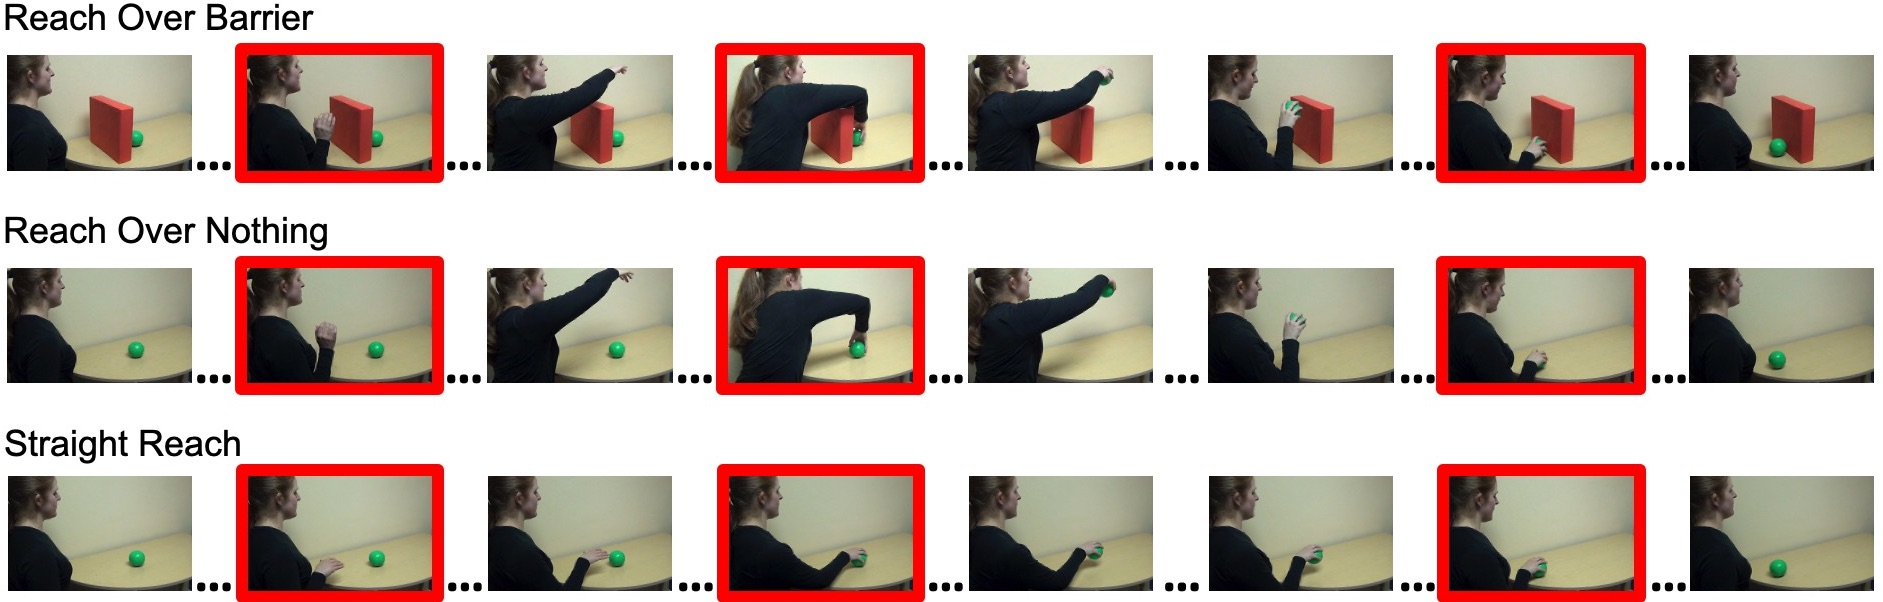
\includegraphics[width=6.28in]{figures/slide_examples}

\}

\textbackslash caption\{Examples of boundary and non-boundary slides from the \emph{barrier}, \emph{nothing}, and \emph{straight} slideshows. Boundary slides are outlined in red.\}\label{fig:fig1}
\textbackslash end\{figure\}

\hypertarget{motion-change}{%
\subsection{Motion Change}\label{motion-change}}

To gain an objective measure of motion-pattern differences across slideshows, we calculated pixel change as an index of slide-to-slide motion change in each of the three slideshows (following Hard et al., 2011). A Canny Edge Detector convolution filter (Canny, 1986) identified and highlighted high contrast areas of each slide image. These areas correspond to the edges of people and objects (see Figure 2). We then calcuated the degree of pixel change between adjacent convolution-filtered frames (Loucks and Baldwin (2009); see OSF repository for further details). The resulting values indicated the average amount of pixel change between a given slide and the slide immediately preceding it.

\textbackslash begin\{figure\}

\{\centering 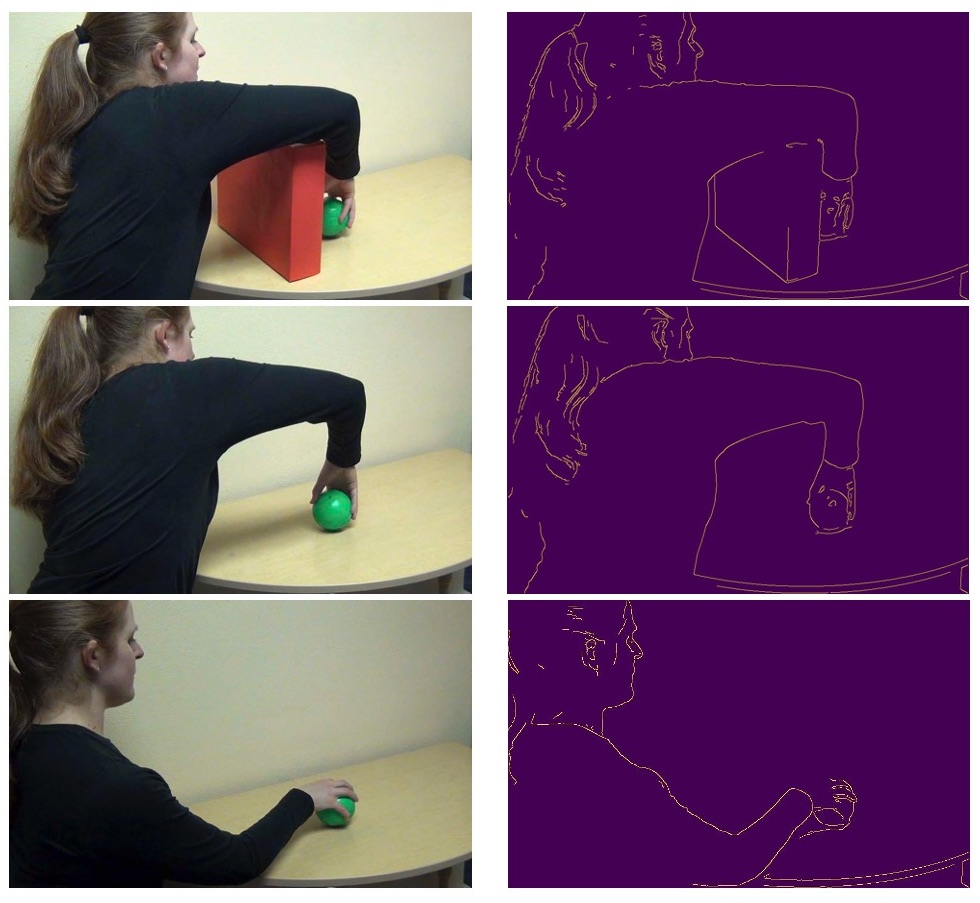
\includegraphics[width=4in]{figures/convolution_filtered}

\}

\textbackslash caption\{Examples of what original slides looked like for the \emph{barrier} (top), \emph{nothing} (middle), and \emph{straight} (bottom) slideshows before (left) and after (right) being passed through a convolution filter.\}\label{fig:fig2}
\textbackslash end\{figure\}

An analysis of variance revealed that overall average pixel change values differed across the \emph{barrier} (\emph{M} =7.73, \emph{SD} = 0.91), \emph{nothing} (\emph{M} = 7.53, \emph{SD} = 1.60), and \emph{straight} slideshows (\emph{M} = 4.91, \emph{SD} = 0.54), \(F(2, 48) = 36.73\), \(p< .001\). A set of Bonferroni-correct pairwise comparisons confirmed that this difference was primarily driven by relatively lower pixel change across the \emph{straight} slideshow. Average pixel change was lower for the \emph{straight} slideshow than both the \emph{barrier} or \emph{nothing} slideshows (ps = \textless{} .001 and \textless{} .001, respectively). Average pixel change did not differ between the \emph{barrier} and \emph{nothing} slideshows (\(p=> .999\)). The difference in pixel change for boundary versus non-boundary slides did not reach statistical signifiance, \(F(1, 48) = 3.02\), \(p =.089\), nor was there a significant interaction between condition and slide type,\(F(2, 48) = 0.27\), \(p =0.76\). Thus, if a boundary advantage effect were observed in subsequent analyses, it would be unlikely that this effect could be solely explained by differences in motion change between boundary and non-boundary slides.

Figure 3 illustrates these similarities and differences in pixel change. While there were overall differences in the magnitude of absolute pixel change between conditions, the general patterns of pixel change were similar for the \emph{barrier} and \emph{nothing} slideshows, but differed between each of these conditions relative to thethe \emph{straight} reach slideshow. Because the \emph{barrier} and \emph{nothing} reaches unfolded in the same manner (arcing up and over) while the \emph{straight} reach did not, these patterns were precisely what would be expected.

\textbackslash begin\{figure\}

\{\centering 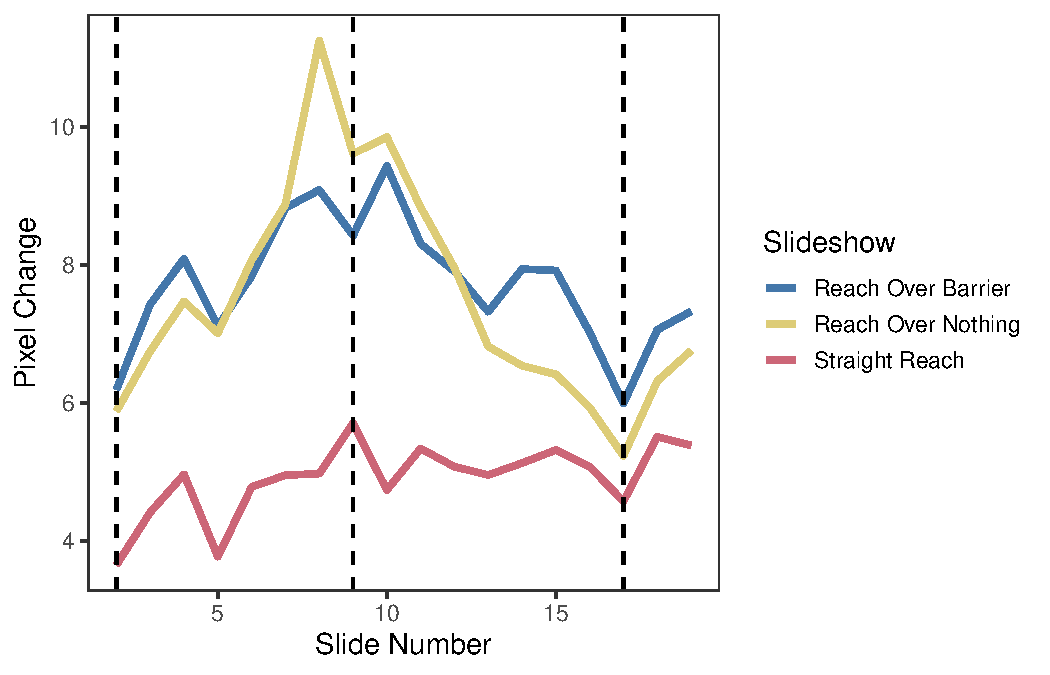
\includegraphics{kg-paper_files/figure-latex/fig3-1}

\}

\textbackslash caption\{Degree of absolute pixel change across the \emph{barrier}, \emph{nothing}, and \emph{straight} reach slideshows. Dashed lines indicate slides corresponding to event boundaries.\}\label{fig:fig3}
\textbackslash end\{figure\}

\hypertarget{procedure}{%
\subsection{Procedure}\label{procedure}}

After consenting, parents were seated in a screened-off corner of the study room and asked to remain quiet throughout the session. Children were invited to take a seat at the computer equipped with a wired mouse; a prominent sticker on the mouse indicated where to click. The experiment consisted of a training task and then the main dwell-time task (see OSF repository for additional details of instructions and procedure). The goal of the training task (a slideshow depicting a train moving from right to left across the screen) was simply to acquaint children with the experience of clicking the mouse to advance slides in order to see an event unfold. After completing the training task, children then clicked through one of the three slideshows. After viewing the slideshow once, an image of a field and clouds was presented, and children then immediately clicked through the same slideshow a second time.

Participants' dwell times (i.e., latency between one mouse click and the next) were recorded using Psychtoolbox (Brainard, 1997), a Matlab© toolbox designed to optimize presentation of visual stimuli. The dwell time task was programmed such that children could only advance slides forward; review of previous slides was not possible.

\hypertarget{results}{%
\section{Results}\label{results}}

\hypertarget{preparing-dwell-time-data}{%
\subsection{Preparing Dwell Time Data}\label{preparing-dwell-time-data}}

As described previously, dwell times index the latency between mouse clicks, or the total amount of time a given slide was visible on the screen. We used standard methods to prepare dwell-time data for analyses (e.g., Kosie \& Baldwin, 2019b, 2019a). As is typical of reaction time data (dwell time data included), dwell times in the current study were positively skewed. Thus, all dwell times were first log\textsubscript{10} transformed to normalize the distribution prior to analyses. Log\textsubscript{10} transformed dwell times greater than three standard deviations above the overall group mean were considered outliers. When more than 10\% of any one participants' data met this outlier criterion, that participant's data were excluded from further analyses. In the current study, three participants' data were excluded for this reason, leaving 89 total participants (N\textsubscript{barrier} = 31, N\textsubscript{nothing} = 25, N\textsubscript{straight} = 30). Remaining dwell times that met this outlier criterion (1.6\% of the data) were Winsorized (Tukey, 1977); specifically, outlying dwell times were replaced with the dwell time value representing three standard deviations above the group mean.

We fit linear mixed effects models with type III sums of squares using the \texttt{lme4} package (Bates, Maechler, Bolker, \& Walker, 2015) in R (Team, 2019). The \texttt{lmerTest} package (Kuznetsova, Brockhoff, \& Christensen, 2017) was used to assess statistical significance using Satterthwaite's approximation for degrees of freedom.

In a preliminary analysis, we first asked whether there were systamatic dwell-time differences across preschoolers' viewings of the same slideshow and whether this effect differed across the three slideshow versions. To test this, we ran a mixed-effects model predicting dwell time from fixed effects of viewing and slideshow, random intecepts for subjects, and random slopes for viewing. This analysis revealed that, while overall average dwell times decreased significantly from first to second viewing (\(F(1, 83.00) = 4.23\), \(p = .043\)), this effect did not interact with slideshow (\(F(2, 83.00) = 0.68\), \(p = .512\)). Because the overall decline in dwell time from first to second viewing was similar across all three slideshows, dwell times were averaged across the two viewings.

\hypertarget{preschoolers-priortized-segmental-structure-over-motion-trajectory.}{%
\subsection{Preschoolers priortized segmental structure over motion trajectory.}\label{preschoolers-priortized-segmental-structure-over-motion-trajectory.}}

In our first analysis, we we examined the extent to which slide type (boundary vs.~non-boundary), slideshow ( \emph{barrier} vs.~\emph{nothing} vs.~\emph{straight}), and their interaction related to participants' dwell times. In this mixed-effects model we predicted dwell time from fixed effects for slide type and condition, random intercepts for subjects, and random slopes for slide type. Replicating previous work with preschoolers and adults (e.g., Meyer et al., 2011; Hard et al., 2011; Kosie \& Baldwin, 2019b, 2019a; Ross \& Baldwin, 2015), preschoolers' dwell times were significantly longer to boundary (\emph{M} = 2.89, \emph{SD} = 0.21) over non-boundary slides (\emph{M} = 2.84, \emph{SD} = 0.20), \(\beta=0.02\) (\(SE=0.01\), \(p= < .001\). Neither slideshow nor the interaction between slide type and slideshow were significant predictors of dwell time, all \(ps >= 0.89\). Thus, despite observed differences in motion trajectory across the three slideshows, preschoolers' attentional patterns indicated that they prioritize goal structure over lower-level motion parameters as they processed dynamically unfolding sequences.

To further test the extent to which motion patterns influenced preschoolers' dwell times, slide-to-slide pixel change was included as a covariate in the above-described model. Pixel change was not a significant preditor of participants' dwell times, \(\beta=0.00\) (\(SE=0.00\), \(p=.516\). Additionally, when including pixel change as a covariate, the overall pattern of results did not change; slide type remained the only significant predictor of dwell time, \(\beta=0.02\) (\(SE=0.01\), \(p=< .001\). These results, which can be seen in Figure 4, are consistent with the hypothesis that goal structure is a primary determinant of preschoolers' segmental analysis of continuously unfolding dynamic activity.

\textbackslash begin\{figure\}

\{\centering 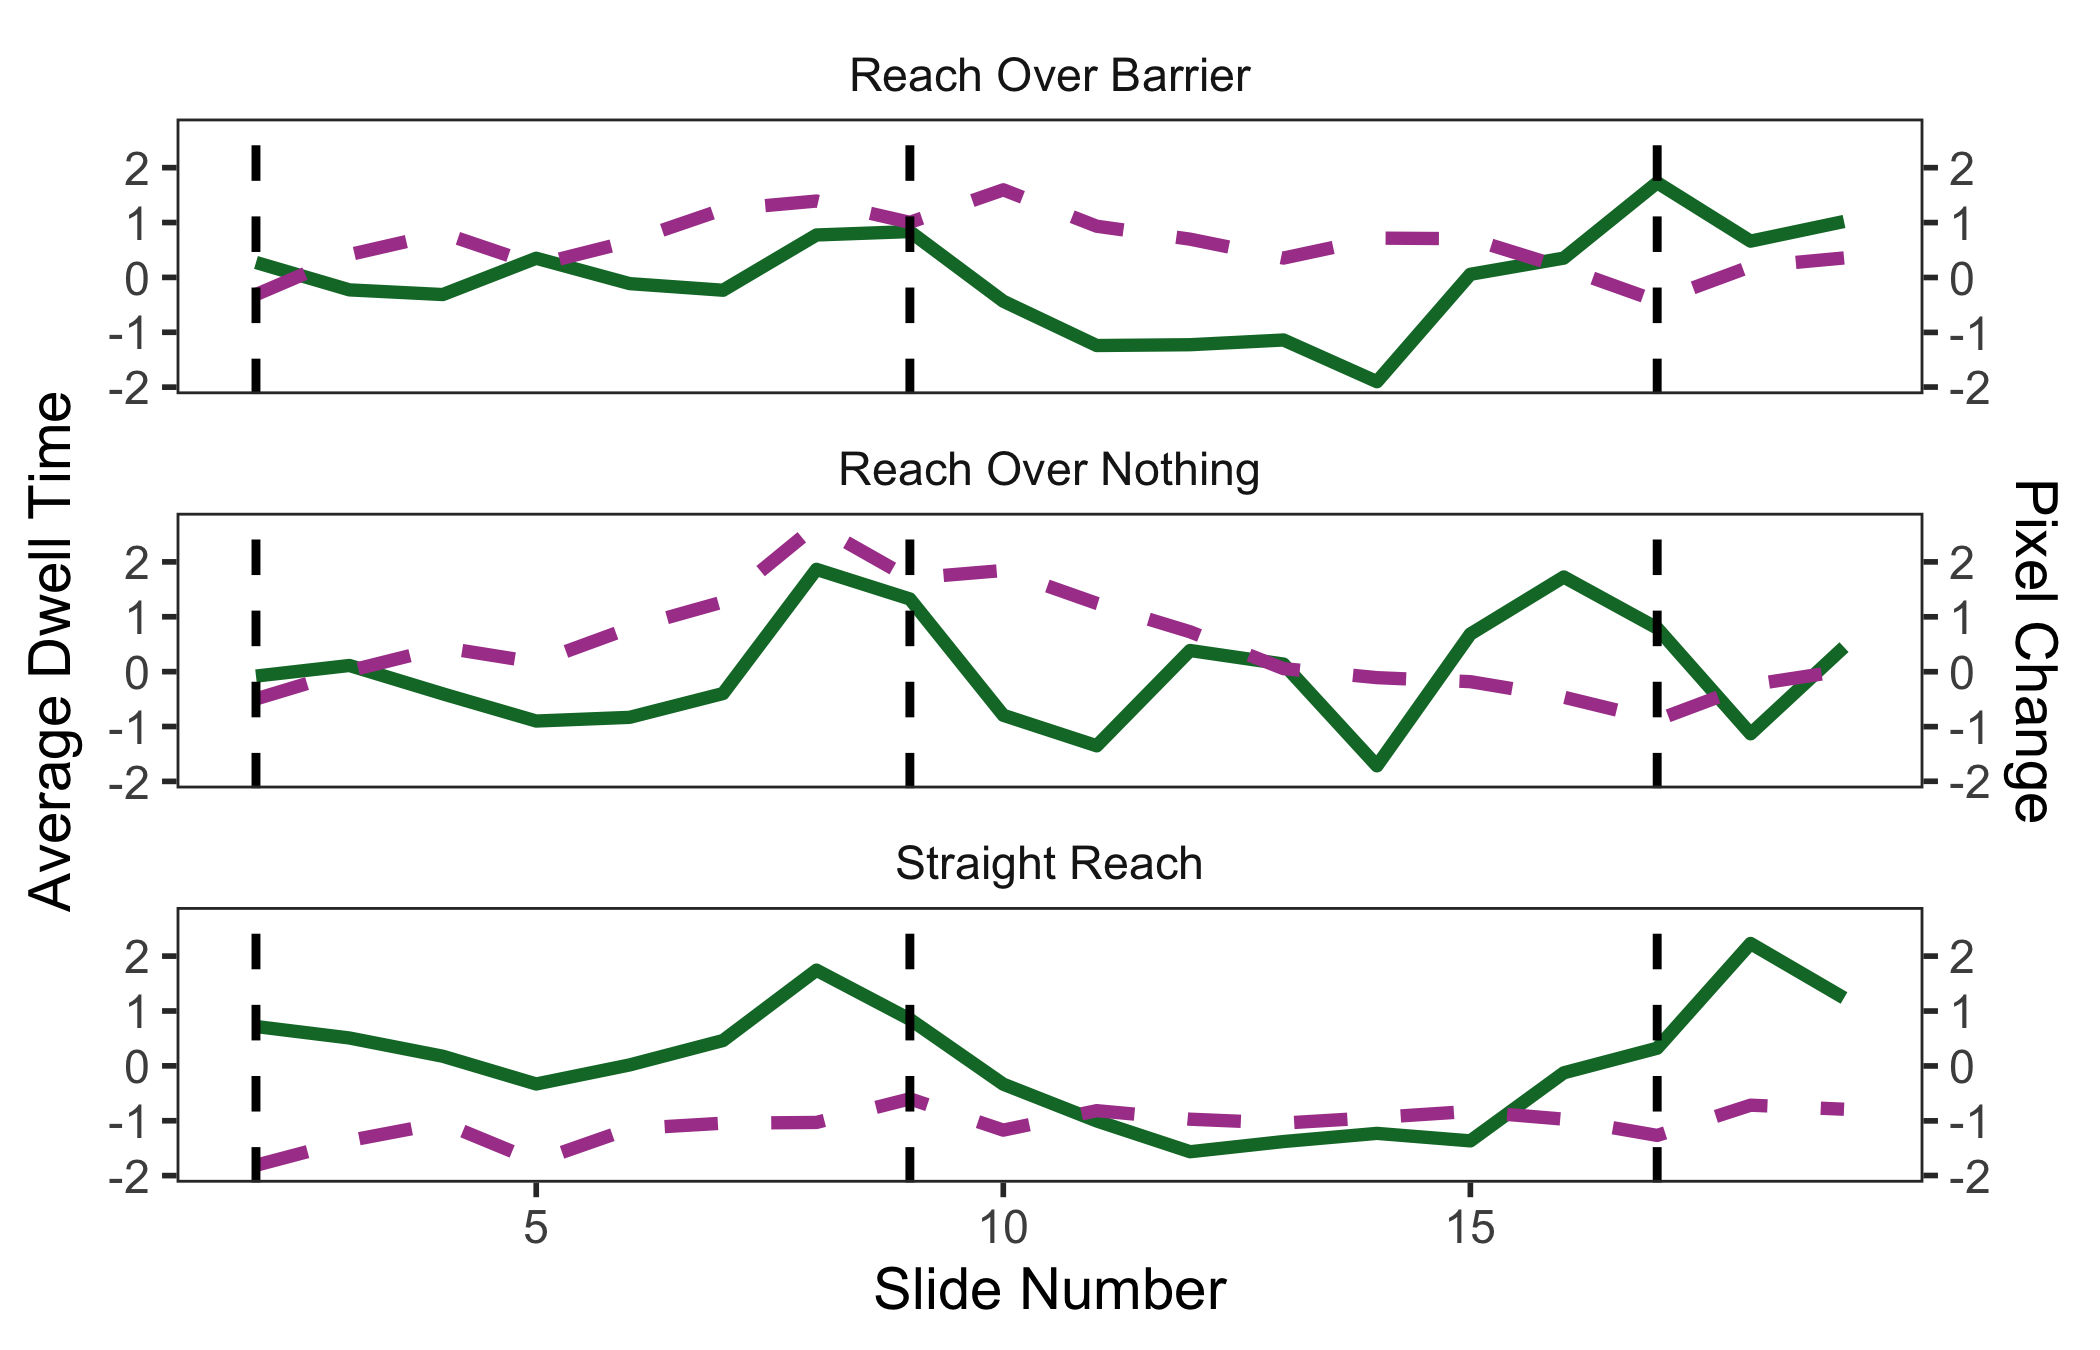
\includegraphics{kg-paper_files/figure-latex/fig4-1}

\}

\textbackslash caption\{Dwell times (red, left axis) and pixel change (blue, right axis) across the \emph{barrier}, \emph{nothing}, and \emph{straight} slideshows. Dashed lines indicate event boundaries. Both dwell times and pixel change are z-scored to aid in interpretability.\}\label{fig:fig4}
\textbackslash end\{figure\}

\hypertarget{exploratory-analyses-revealed-an-increase-in-attention-to-causal-violations.}{%
\subsection{Exploratory analyses revealed an increase in attention to causal violations.}\label{exploratory-analyses-revealed-an-increase-in-attention-to-causal-violations.}}

While we did not find an overall significant effect of condition or pixel change, visual inspection of Figure 4 revealed a surge in mean dwell time between slides 12 and 13 of the \emph{nothing} slideshow that seemed to be absent in the other two slideshows. This region corresponds to the juncture in the \emph{nothing} slideshow at which the actor uses an arcing reach - despite the absence of a barrier - to bring the ball back and place it on the table in front of her. If, as described earlier, preschoolers are sensitive to this violation of the canonical properties of goal-oriented action, this juncture might be where we would anticipate a corresponding violation/novelty-related increase in dwell times (as has been observed in previous dwell-time studies with adults; Sage \& Baldwin, 2014; Kosie \& Baldwin, 2019b). If the effect were quite large, we would have observed it in our earlier analysis, reported above, comparing participants' dwell times across the three slideshows. However, it is possible that small but nevertheless systematic differences could be observable between the \emph{nothing} versus \emph{barrier} and \emph{straight} slideshows. if analyses were to focus narrowly on the relevant region - where the violation of canonical action specifically occurred Thus, we next compared participants' dwell times within this region of causal violation across the \emph{barrier}, \emph{nothing}, and \emph{straight} slideshows (slides 12-13). Because decisions regarding which slides to include in analyses were made \emph{after} viewing Figure 4, we conducted and interpreted these analyses in a purely exploratory manner. Numerically, mean dwell times were greater to the region of causal violation in the \emph{nothing} condition (\emph{M} = 2.87, \emph{SD} = 0.25) than in the \emph{barrier} (\emph{M} = 2.79, \emph{SD} = 0.16) or \emph{straight} conditions (\emph{M} = 2.78, \emph{SD} = 0.15). However, neither the omnibus test of condition nor direct comparisons between the \emph{nothing}, \emph{barrier}, and \emph{straight} conditions reached statistical significance, all \(ps >=0.06\). While the differences in means were suggestive that preschoolers - like the infants' in Phillips and Wellman's (2005) research - may be sensitive to violations to canonical goal-oriented action, clear conclusions to this effect could not be drawn from the current results.

\hypertarget{discussion}{%
\section{Discussion}\label{discussion}}

Although prior research clarifies that young children often weight goal structure information more heavily than motion patterns in their interpretation and memory for human actions, it wasn't known how these two sources of information influence children's segmental analysis as activity unfolds across time. To this effect, we examined the extent to which children's knowledge of goal structure influenced their segmental analysis of unfolding behavior, relative to the influence of differential motion patterns. Preschoolers advanced at their own pace (via the dwell time paradigm) through slideshows depicting three activity sequences. The three sequences had the same goal-related segmental structure, but differed in motion parameters. As preschoolers viewed the sequences, we measured their time spent ``dwelling'' on each slide, an index of attentional allocation. Across all three activity sequences, preschoolers' dwell times increased at event boundaries, or junctures at which one unit of action ended and another began. These results - using three new activity sequences - replicate previous research, and suggest that preschoolers, like adults, attend to goal-related segmental structure as they process unfolding activity (Hard, Meyer, \& Baldwin, 2019; Hard et al., 2011; Kosie \& Baldwin, 2019b, 2019a; Meyer et al., 2011; Ross \& Baldwin, 2015).

We additionally engaged in several analyses to explore the extent to which preschoolers' dwell time patterns tracked the motion parameters of each sequence. First, we demonstrated that the observed boundary advantage did not differ across the three reaching conditions, suggesting that the boundary advantage is robust to variation in the precise path an actor takes to achieve a goal. Next, we found that slide-to-slide pixel change - an index of changes in degree of physical motion for each individual slide - were also not predictive of preschoolers' dwell times. Finally, while we saw some indication that preschoolers up-regulated attention to a causal violation (e.g., Phillips \& Wellman, 2005; Sage \& Baldwin, 2014), this effect was weak and did not reach statistical significance. In sum, these results provide substantial evidence that goal-related segmental structure, rather than the specifics of motion parameters underlying the activity stream, are a primary determinant of preschoolers' dwell time patterns.

In addition to providing new insight into how preschoolers modulate their attention when viewing everyday action, this work validated the dwell-time paradigm as a useful methodology with which to explore preschoolers' processing of activity as it unfolds. The dwell-time paradigm is inexpensive, child-friendly, easy to use, and portable. Thus, in addition to use in the lab, this paradigm can be implemented in preschools, museums, and in the field. We are currently working to develop a version that can be used online, expanding our ability to recruit a large and diverse sample. Finally, because the dwell time paradigm is an implicit measure of processing - requiring only that participants click through an unfolding slideshow - it provides the opportunity to run exactly the same experiment with adults and children. Comparing the dwell times of children and adults enables us to explore differences in processing across these two groups and holds potential to reveal nuanced information about how children's processing becomes more adult-like over time.

In conclusion, we (a) replicated previous findings that preschoolers, like adults, attend to action's goal-related segmental structure, (b) extended these findings to demonstrate that preschoolers prioritize goal structure over motion properties in their segmental analysis of activity streams, and (c) showcased the value of the dwell time paradigm as a useful methodology with which to investigate preschoolers' processing of dynamically unfolding visual information. These results set the stage for further investigation into factors that influence preschoolers' processing of events as their development and knowledge acquision progress.

\hypertarget{footnote}{%
\section{Footnote?}\label{footnote}}

In adult dwell time studies, dwell times typically show a power curve indicative of partcipants speeding up as they view the slideshow, and a residulization procedure is typically used to correct for this power curve (see Hard et al., 2011; Kosie \& Baldwin, 2019b for more detail regarding this process). In the current study, however, only XX\% of participants' dwell times fit a significant power curve. This suggests that, unlike adults, preschoolers did not speed up as they viewed the slideshows. This is perhaps because the slideshows in the current study were quite short (e.g., 20 slides versus over 100 slides in typical slideshows viewed by adults). Thus, we opted to use log\textsubscript{10} dwell times (henceforth, ``dwell times'') in all analyses rather than carrying out the residualization procedure. ***I'm unsure how to look for the power curve - separately for each slideshow? Do I need to report power curve?

\newpage

\hypertarget{references}{%
\section{References}\label{references}}

\begingroup
\setlength{\parindent}{-0.5in}
\setlength{\leftskip}{0.5in}

\hypertarget{refs}{}
\begin{cslreferences}
\leavevmode\hypertarget{ref-bailey_2013}{}%
Bailey, H. R., Kurby, C. A., Giovannetti, T., \& Zacks, J. M. (2013). Action perception predicts action performance. \emph{Neuropsychologia}, \emph{51}(11), 2294--2304. doi:\href{https://doi.org/10.1016/j.neuropsychologia.2013.06.022}{10.1016/j.neuropsychologia.2013.06.022}

\leavevmode\hypertarget{ref-baldassano_2017}{}%
Baldassano, C., Chen, J., Zadbood, A., Pillow, J. W., Hasson, U., \& Norman, K. A. (2017). Discovering Event Structure in Continuous Narrative Perception and Memory. \emph{Neuron}, \emph{95}(3), 709--721.e5. doi:\href{https://doi.org/10.1016/j.neuron.2017.06.041}{10.1016/j.neuron.2017.06.041}

\leavevmode\hypertarget{ref-baldwin_2012}{}%
Baldwin, D. A. (2012). Redescribing action. In \emph{Navigating the social world: What infants, children, and other species can teach us.} New York: Oxford University Press.

\leavevmode\hypertarget{ref-baldwin_baird_1999}{}%
Baldwin, D. A., \& Baird, J. A. (1999). Action analysis: A gateway to intentional inference. In \emph{Early social cognition: Understanding others in the first months of life} (pp. 215--240). Mahwah, NJ: Lawrence Earlbaum Associates.

\leavevmode\hypertarget{ref-baldwin_baird_2001}{}%
Baldwin, D. A., \& Baird, J. A. (2001). Discerning intentions in dynamic human action. \emph{Trends in Cognitive Sciences}, \emph{5}(4), 171--178. doi:\href{https://doi.org/10.1016/S1364-6613(00)01615-6}{10.1016/S1364-6613(00)01615-6}

\leavevmode\hypertarget{ref-baldwin_2001}{}%
Baldwin, D. A., Baird, J. A., Saylor, M. M., \& Clark, M. A. (2001). Infants Parse Dynamic Action. \emph{Child Development}, \emph{72}(3), 708--717. doi:\href{https://doi.org/10.1111/1467-8624.00310}{10.1111/1467-8624.00310}

\leavevmode\hypertarget{ref-baldwin_2008}{}%
Baldwin, D., Andersson, A., Saffran, J., \& Meyer, M. (2008). Segmenting dynamic human action via statistical structure. \emph{Cognition}, \emph{106}(3), 1382--1407. doi:\href{https://doi.org/10.1016/j.cognition.2007.07.005}{10.1016/j.cognition.2007.07.005}

\leavevmode\hypertarget{ref-bates_2015}{}%
Bates, D., Maechler, M., Bolker, B., \& Walker, S. (2015). Fitting linear mixed effects models using lme4. \emph{Journal of Statistical Software}, \emph{67}(1), 1--48. doi:\href{https://doi.org/10.18637/jss.v067.i01}{10.18637/jss.v067.i01}

\leavevmode\hypertarget{ref-brainard_1997}{}%
Brainard, D. H. (1997). The Psychophysics Toolbox. \emph{Spatial Vision}, \emph{10}(4), 433--436. doi:\href{https://doi.org/10.1163/156856897X00357}{10.1163/156856897X00357}

\leavevmode\hypertarget{ref-buresh_woodward_2007}{}%
Buresh, J. S., \& Woodward, A. L. (2007). Infants track action goals within and across agents. \emph{Cognition}, \emph{104}(2), 287--314. doi:\href{https://doi.org/10.1016/j.cognition.2006.07.001}{10.1016/j.cognition.2006.07.001}

\leavevmode\hypertarget{ref-canny_1986}{}%
Canny, J. (1986). A Computational Approach to Edge Detection. \emph{IEEE Transactions on Pattern Analysis and Machine Intelligence}, \emph{6}, 679--698.

\leavevmode\hypertarget{ref-falckytter_2006}{}%
Falck-Ytter, T., Gredebäck, G., \& Hofsten, C. von. (2006). Infants predict other people's action goals. \emph{Nature Neuroscience}, \emph{9}(7), 878--879. doi:\href{https://doi.org/10.1038/nn1729}{10.1038/nn1729}

\leavevmode\hypertarget{ref-gergely_csibra_2003}{}%
Gergely, G., \& Csibra, G. (2003). Teleological reasoning in infancy: The naı̈ve theory of rational action. \emph{Trends in Cognitive Sciences}, \emph{7}(7), 287--292. doi:\href{https://doi.org/10.1016/S1364-6613(03)00128-1}{10.1016/S1364-6613(03)00128-1}

\leavevmode\hypertarget{ref-gergely_1995}{}%
Gergely, G., Nádasdy, Z., Csibra, G., \& Bíró, S. (1995). Taking the intentional stance at 12 months of age. \emph{Cognition}, \emph{56}(2), 165--193. doi:\href{https://doi.org/10.1016/0010-0277(95)00661-H}{10.1016/0010-0277(95)00661-H}

\leavevmode\hypertarget{ref-gredeback_melinder_2010}{}%
Gredebäck, G., \& Melinder, A. (2010). Infants' understanding of everyday social interactions: A dual process account. \emph{Cognition}, \emph{114}(2), 197--206. doi:\href{https://doi.org/10.1016/j.cognition.2009.09.004}{10.1016/j.cognition.2009.09.004}

\leavevmode\hypertarget{ref-hard_2018}{}%
Hard, B. M., Meyer, M., \& Baldwin, D. (2019). Attention reorganizes as structure is detected in dynamic action. \emph{Memory \& Cognition}, \emph{47}(1), 17--32. doi:\href{https://doi.org/10.3758/s13421-018-0847-z}{10.3758/s13421-018-0847-z}

\leavevmode\hypertarget{ref-hard_2011}{}%
Hard, B. M., Recchia, G., \& Tversky, B. (2011). The shape of action. \emph{Journal of Experimental Psychology: General}, \emph{140}(4), 586--604. doi:\href{https://doi.org/10.1037/a0024310}{10.1037/a0024310}

\leavevmode\hypertarget{ref-hespos_2010}{}%
Hespos, S. J., Grossman, S. R., \& Saylor, M. M. (2010). Infants' ability to parse continuous actions: Further evidence. \emph{Neural Networks}, \emph{23}(8-9), 1026--1032. doi:\href{https://doi.org/10.1016/j.neunet.2010.07.010}{10.1016/j.neunet.2010.07.010}

\leavevmode\hypertarget{ref-hespos_2009}{}%
Hespos, S. J., Saylor, M. M., \& Grossman, S. R. (2009). Infants' ability to parse continuous actions. \emph{Developmental Psychology}, \emph{45}(2), 575--585. doi:\href{https://doi.org/10.1037/a0014145}{10.1037/a0014145}

\leavevmode\hypertarget{ref-kosie_baldwin_2019b}{}%
Kosie, J. E., \& Baldwin, D. (2019a). Attentional profiles linked to event segmentation are robust to missing information. \emph{Cognitive Research: Principles and Implications}, \emph{4}(1), 8. doi:\href{https://doi.org/10.1186/s41235-019-0157-4}{10.1186/s41235-019-0157-4}

\leavevmode\hypertarget{ref-kosie_baldwin_2019a}{}%
Kosie, J. E., \& Baldwin, D. (2019b). Attention rapidly reorganizes to naturally occurring structure in a novel activity sequence. \emph{Cognition}, \emph{182}, 31--44. doi:\href{https://doi.org/10.1016/j.cognition.2018.09.004}{10.1016/j.cognition.2018.09.004}

\leavevmode\hypertarget{ref-kosie_baldwin_OSF}{}%
Kosie, J. E., \& Baldwin, D. A. (2020). OSF Repository: Dwell times disambiguate preschoolers' attention to motion versus goal structure as dynamic action unfolds. \emph{Open Science Framework}. Retrieved from \url{doi:\%2010.17605/OSF.IO/M6Q7R}

\leavevmode\hypertarget{ref-kurby_zacks_2008}{}%
Kurby, C. A., \& Zacks, J. M. (2008). Segmentation in the perception and memory of events. \emph{Trends in Cognitive Sciences}, \emph{12}(2), 72--79. doi:\href{https://doi.org/10.1016/j.tics.2007.11.004}{10.1016/j.tics.2007.11.004}

\leavevmode\hypertarget{ref-kurby_zacks_2011}{}%
Kurby, C. A., \& Zacks, J. M. (2011). Age differences in the perception of hierarchical structure in events. \emph{Memory \& Cognition}, \emph{39}(1), 75--91. doi:\href{https://doi.org/10.3758/s13421-010-0027-2}{10.3758/s13421-010-0027-2}

\leavevmode\hypertarget{ref-lmerTest}{}%
Kuznetsova, A., Brockhoff, P. B., \& Christensen, R. H. B. (2017). Package: Tests in Linear Mixed Effects Models. \emph{Journal of Statistical Software}, \emph{82}(13), 1--26. doi:\href{https://doi.org/10.18637/jss.v082.i13}{10.18637/jss.v082.i13}

\leavevmode\hypertarget{ref-loucks_baldwin_2009}{}%
Loucks, J., \& Baldwin, D. (2009). Sources of information for discriminating dynamic human actions. \emph{Cognition}, \emph{111}(1), 84--97. doi:\href{https://doi.org/10.1016/j.cognition.2008.12.010}{10.1016/j.cognition.2008.12.010}

\leavevmode\hypertarget{ref-meltzoff_1995}{}%
Meltzoff, A. N. (1995). Understanding the intentions of others: Re-enactment of intended acts by 18-month-old children. \emph{Developmental Psychology}, \emph{31}(5), 838--850.

\leavevmode\hypertarget{ref-meyer_2011}{}%
Meyer, M., Baldwin, D. A., \& Sage, K. D. (2011). Assessing Young Children's Hierarchical Action Segmentation. \emph{Proceedings of the Cognitive Science Society}, \emph{33}, 3156--3161.

\leavevmode\hypertarget{ref-newtson_1973}{}%
Newtson, D. (1973). Attribution and the unit of perception of ongoing behavior. \emph{Journal of Personality and Social Psychology}, \emph{28}(1), 28--38. doi:\href{https://doi.org/10.1037/h0035584}{10.1037/h0035584}

\leavevmode\hypertarget{ref-newtson_1977}{}%
Newtson, D., Engquist, G., \& Bois, J. (1977). The Objective Basis of Behavior Units. \emph{Journal of Personality and Social Psychology}, \emph{35}(12), 847--862.

\leavevmode\hypertarget{ref-olofson_baldwin_2011}{}%
Olofson, E. L., \& Baldwin, D. (2011). Infants recognize similar goals across dissimilar actions involving object manipulation. \emph{Cognition}, \emph{118}(2), 258--264. doi:\href{https://doi.org/10.1016/j.cognition.2010.11.012}{10.1016/j.cognition.2010.11.012}

\leavevmode\hypertarget{ref-pace_2020}{}%
Pace, A., Levine, D. F., Golinkoff, R. M., Carver, L. J., \& Hirsh-Pasek, K. (2020). Keeping the end in mind: Preliminary brain and behavioral evidence for broad attention to endpoints in pre-linguistic infants. \emph{Infant Behavior and Development}, \emph{58}, 101425. doi:\href{https://doi.org/10.1016/j.infbeh.2020.101425}{10.1016/j.infbeh.2020.101425}

\leavevmode\hypertarget{ref-phillips_wellman_2005}{}%
Phillips, A. T., \& Wellman, H. M. (2005). Infants' understanding of object-directed action. \emph{Cognition}, \emph{98}(2), 137--155. doi:\href{https://doi.org/10.1016/j.cognition.2004.11.005}{10.1016/j.cognition.2004.11.005}

\leavevmode\hypertarget{ref-phillips_2002}{}%
Phillips, A. T., Wellman, H. M., \& Spelke, E. S. (2002). Infants' ability to connect gaze and emotional expression to intentional action. \emph{Cognition}, \emph{85}(1), 53--78. doi:\href{https://doi.org/10.1016/S0010-0277(02)00073-2}{10.1016/S0010-0277(02)00073-2}

\leavevmode\hypertarget{ref-ross_baldwin_2015}{}%
Ross, R. A., \& Baldwin, D. A. (2015). Event processing as an executive enterprise. In \emph{Emerging trends in the social and behavioral sciences: An interdisciplinary, searchable, and linkable resource.} (pp. 1--13).

\leavevmode\hypertarget{ref-sage_baldwin_2014}{}%
Sage, K. D., \& Baldwin, D. (2014). Looking to the hands: Where we dwell in complex manual sequences. \emph{Visual Cognition}, \emph{22}(8), 1092--1104. doi:\href{https://doi.org/10.1080/13506285.2014.962123}{10.1080/13506285.2014.962123}

\leavevmode\hypertarget{ref-sage_baldwin_2015}{}%
Sage, K. D., \& Baldwin, D. (2015). Children's Use of Self-Paced Slideshows: An Extension of the Video Deficit Effect? \emph{Journal of Research in Childhood Education}, \emph{29}(1), 90--114. doi:\href{https://doi.org/10.1080/02568543.2014.978919}{10.1080/02568543.2014.978919}

\leavevmode\hypertarget{ref-sargent_2013}{}%
Sargent, J. Q., Zacks, J. M., Hambrick, D. Z., Zacks, R. T., Kurby, C. A., Bailey, H. R., \ldots{} Beck, T. M. (2013). Event segmentation ability uniquely predicts event memory. \emph{Cognition}, \emph{129}(2), 241--255. doi:\href{https://doi.org/10.1016/j.cognition.2013.07.002}{10.1016/j.cognition.2013.07.002}

\leavevmode\hypertarget{ref-saylor_2007}{}%
Saylor, M. M., Baldwin, D. A., Baird, J. A., \& LaBounty, J. (2007). Infants' On-line Segmentation of Dynamic Human Action. \emph{Journal of Cognition and Development}, \emph{8}(1), 113--128. doi:\href{https://doi.org/10.1080/15248370709336996}{10.1080/15248370709336996}

\leavevmode\hypertarget{ref-sonne_2016}{}%
Sonne, T., Kingo, O. S., \& Krøjgaard, P. (2016). Occlusions at event boundaries during encoding have a negative effect on infant memory. \emph{Consciousness and Cognition}, \emph{41}, 72--82. doi:\href{https://doi.org/10.1016/j.concog.2016.02.006}{10.1016/j.concog.2016.02.006}

\leavevmode\hypertarget{ref-sonne_2017}{}%
Sonne, T., Kingo, O. S., \& Krøjgaard, P. (2017). Bound to remember: Infants show superior memory for objects presented at event boundaries. \emph{Scandinavian Journal of Psychology}, \emph{58}(2), 107--113. doi:\href{https://doi.org/10.1111/sjop.12351}{10.1111/sjop.12351}

\leavevmode\hypertarget{ref-stahl_2014}{}%
Stahl, A. E., Romberg, A. R., Roseberry, S., Golinkoff, R. M., \& Hirsh-Pasek, K. (2014). Infants Segment Continuous Events Using Transitional Probabilities. \emph{Child Development}, n/a--n/a. doi:\href{https://doi.org/10.1111/cdev.12247}{10.1111/cdev.12247}

\leavevmode\hypertarget{ref-swallow_zacks_2008}{}%
Swallow, K. M., \& Zacks, J. M. (2008). Sequences learned without awareness can orient attention during the perception of human activity. \emph{Psychonomic Bulletin \& Review}, \emph{15}(1), 116--122. doi:\href{https://doi.org/10.3758/PBR.15.1.116}{10.3758/PBR.15.1.116}

\leavevmode\hypertarget{ref-r}{}%
Team, R. C. (2019). R: A Language and Environment for Statistical Computing. Vienna, Austria: R Foundation for Statitsical Computing. Retrieved from \url{https://www.R-project.org/}

\leavevmode\hypertarget{ref-tukey_1977}{}%
Tukey, J. W. (1977). \emph{Exploratory Data Analysis}. Massachusetts: Addison-Wesley.

\leavevmode\hypertarget{ref-woodward_1998}{}%
Woodward, A. (1998). Infants selectively encode the goal object of an actor's reach. \emph{Cognition}, \emph{69}(1), 1--34. doi:\href{https://doi.org/10.1016/S0010-0277(98)00058-4}{10.1016/S0010-0277(98)00058-4}

\leavevmode\hypertarget{ref-woodward_2009}{}%
Woodward, A. L. (2009). Infants' Grasp of Others' Intentions. \emph{Current Directions in Psychological Science}, \emph{18}(1), 53--57. doi:\href{https://doi.org/10.1111/j.1467-8721.2009.01605.x}{10.1111/j.1467-8721.2009.01605.x}

\leavevmode\hypertarget{ref-zacks_2004}{}%
Zacks, J. M. (2004). Using movement and intentions to understand simple events. \emph{Cognitive Science}, \emph{28}(6), 979--1008. doi:\href{https://doi.org/10.1207/s15516709cog2806_5}{10.1207/s15516709cog2806\_5}

\leavevmode\hypertarget{ref-zacks_2007}{}%
Zacks, J. M., Speer, N. K., Swallow, K. M., Braver, T. S., \& Reynolds, J. R. (2007). Event perception: A mind-brain perspective. \emph{Psychological Bulletin}, \emph{133}(2), 273--293. doi:\href{https://doi.org/10.1037/0033-2909.133.2.273}{10.1037/0033-2909.133.2.273}

\leavevmode\hypertarget{ref-zacks_2006a}{}%
Zacks, J. M., Speer, N. K., Vettel, J. M., \& Jacoby, L. L. (2006a). Event understanding and memory in healthy aging and dementia of the Alzheimer type. \emph{Psychology and Aging}, \emph{21}(3), 466--482. doi:\href{https://doi.org/10.1037/0882-7974.21.3.466}{10.1037/0882-7974.21.3.466}

\leavevmode\hypertarget{ref-zacks_2006b}{}%
Zacks, J. M., Swallow, K. M., Vettel, J. M., \& McAvoy, M. P. (2006b). Visual motion and the neural correlates of event perception. \emph{Brain Research}, \emph{1076}(1), 150--162. doi:\href{https://doi.org/10.1016/j.brainres.2005.12.122}{10.1016/j.brainres.2005.12.122}

\leavevmode\hypertarget{ref-zacks_tversky_2001}{}%
Zacks, J. M., \& Tversky, B. (2001). Event Structure in Perception and Conception. \emph{Psychological Bulletin}, \emph{127}(1), 3--21.

\leavevmode\hypertarget{ref-zalla_2013}{}%
Zalla, T., Labruyère, N., \& Georgieff, N. (2013). Perceiving Goals and Actions in Individuals with Autism Spectrum Disorders. \emph{Journal of Autism and Developmental Disorders}, \emph{43}(10), 2353--2365. doi:\href{https://doi.org/10.1007/s10803-013-1784-0}{10.1007/s10803-013-1784-0}
\end{cslreferences}

\endgroup

\end{document}
